\documentclass[tikz,border=10pt]{standalone}
\usepackage{mathabx}
\usepackage{stackengine}
\usetikzlibrary{backgrounds}
\usepackage{newunicodechar}
\newunicodechar{♮}{$\natural$}
\newunicodechar{♭}{$\flat$}
\newunicodechar{♯}{$\sharp$}
\newunicodechar{➚}{$\nearrow$}
\newunicodechar{➘}{$\searrow$}
\newunicodechar{ʼ}{'}
\newunicodechar{Ȧ}{\stackon[0.8pt]{A}{.}}
\newunicodechar{Ḃ}{\stackon[0.8pt]{B}{.}}
\newunicodechar{Ċ}{\stackon[0.8pt]{C}{.}}
\newunicodechar{Ḋ}{\stackon[0.8pt]{D}{.}}
\newunicodechar{Ė}{\stackon[0.8pt]{E}{.}}
\newunicodechar{Ḟ}{\stackon[0.8pt]{F}{.}}
\newunicodechar{Ġ}{\stackon[0.8pt]{G}{.}}


\def\centerarc[#1](#2)(#3:#4:#5);%
{
  \draw[#1]([shift=(#3:#5)]#2) arc (#3:#4:#5);
}


\begin{document}
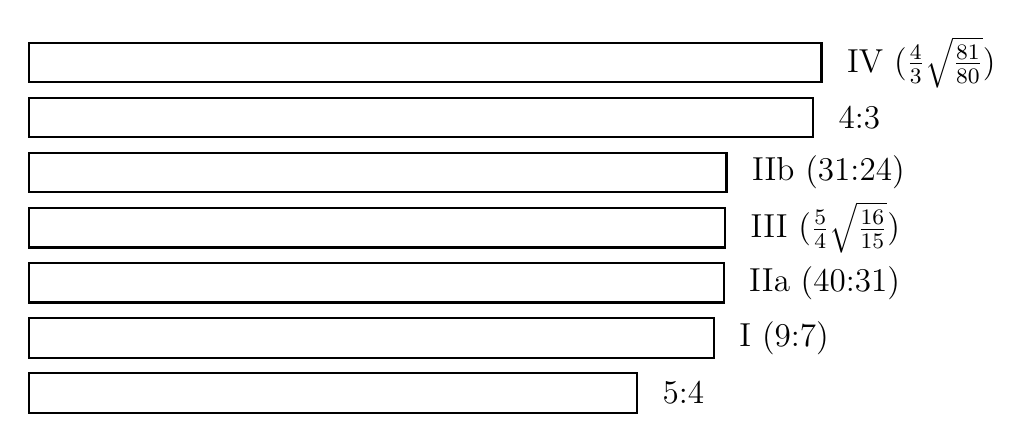
\begin{tikzpicture}

\draw[thick] (0.0, -0.25) -- (7.7260346, -0.25) -- (7.7260346, 0.25) -- (0.0, 0.25) --  cycle;
\node[anchor=west] at (7.9260345, 0.0) { \large 5:4 };
\draw[thick] (0.0, 0.45000002) -- (8.701412, 0.45000002) -- (8.701412, 0.95) -- (0.0, 0.95) --  cycle;
\node[anchor=west] at (8.901412, 0.7) { \large I (9:7) };
\draw[thick] (0.0, 1.15) -- (8.82529, 1.15) -- (8.82529, 1.65) -- (0.0, 1.65) --  cycle;
\node[anchor=west] at (9.0252905, 1.4) { \large IIa (40:31) };
\draw[thick] (0.0, 1.85) -- (8.843313, 1.85) -- (8.843313, 2.3500001) -- (0.0, 2.3500001) --  cycle;
\node[anchor=west] at (9.043313, 2.1000001) { \large III ($\frac{5}{4}\sqrt{\frac{16}{15}}$) };
\draw[thick] (0.0, 2.55) -- (8.861337, 2.55) -- (8.861337, 3.05) -- (0.0, 3.05) --  cycle;
\node[anchor=west] at (9.0613365, 2.8) { \large IIb (31:24) };
\draw[thick] (0.0, 3.25) -- (9.960592, 3.25) -- (9.960592, 3.75) -- (0.0, 3.75) --  cycle;
\node[anchor=west] at (10.160592, 3.5) { \large 4:3 };
\draw[thick] (0.0, 3.95) -- (10.068118, 3.95) -- (10.068118, 4.4500003) -- (0.0, 4.4500003) --  cycle;
\node[anchor=west] at (10.268119, 4.2000003) { \large IV ($\frac{4}{3}\sqrt{\frac{81}{80}}$) };
\end{tikzpicture}
\end{document}